% Author: Bernard Lampe

% Use the IEEE classes
\documentclass[journal]{IEEEtran}

% Packages
\usepackage[cmex10]{amsmath}
\usepackage{url}
\usepackage{cite}
\usepackage{graphicx}
\usepackage{subfig}
\usepackage{float}
\usepackage{amssymb}

% Correct bad hyphenation here
\hyphenation{op-tical net-works semi-conduc-tor}
\DeclareMathOperator*{\argmax}{arg\,max}

% Start document
\begin{document}

% Paper title
\title{Sparse FFT Implementation}

% Author
\author{Bernard~Lampe,~\IEEEmembership{Member,~IEEE}}

% The paper headers
\markboth{Sparse FFT Implementation}
{Shell \MakeLowercase{\Lampe}: Sparse FFT Implementation}

% Make the title area
\maketitle

\begin{abstract}
In this study, we implement the Fast Fourier Transform (FFT) for sparse signals known as the Sparse FFT (SFFT). The goal of this study is to highlight the merits and performance limitations of the algorithm as a function of signal sparsity and signal-to-noise ratio (SNR).
\end{abstract}

% Keywords
\begin{IEEEkeywords}
Fast Fourier Transform, Sparse, FFT, SFFT, Implementation, Performance
\end{IEEEkeywords}

% Introduction with drop letter and first word capitalized.
\section{Introduction}
\IEEEPARstart{W}{e} implemented the sparse fast Fourier transform as outlined in the paper entitled "Simple and Practical Algorithm for Sparse Fourier Transform" by Hassaneih, Indyk, Katabi and Price\cite{hass}. We found the algorithm to be very efficient and effective. The algorithm runs in \(O(klog(k))\) time where \(k\) is the assumed sparsity of the signal. The algorithm outline and run time analysis are detailed in the cited work \cite{hass}. We will briefly summarize the main steps of the algorithm to discuss design choices made in our implementation.

\par To compute the SFFT, the algorithm is broken down into two phases. The first finds the locations of the \(k\) sparse frequencies and the second estimates the frequencies at those locations. The algorithm begins by running what is referred to in the paper as an "location inner loop" \(L = O(log_2(n))\) times. Each iteration of the inner loop will run a \(B\) dimensional FFT where \(B << n\) and divides \(n\). Each iteration of this loop will produce a \(dk\) size set of location votes where \(d\) is the oversample heuristic parameter. These votes are accumulated for each location and when the number of votes for a particular location exceeds \(L/2\) where \(L\) is the number of location loops run. After the location loops are done, "estimation inner loops" are run \(L\) times to compute the possible complex values for each location. The median of these are taken with the real and imaginary parts separate which produces the final estimate for the location.

\par In order to run the \(B\) point FFT in the inner loop, care must be taken to ensure energy from one frequency does not leak into adjacent bins. This is done by employing a tight frequency filter and frequency permutation. The inner loop proceeds by first permuting the time domain samples by a modulus invertible random interval which is co-prime to the data size \(n\). This subsamples the data which permutes the frequency spectrum so that frequencies close together do not clobber each other. Then a time domain filter of size \(w\) is multiplied by the data so that we get a frequency domain convolution to help prevent leakage. The filter used in this implementation is a Gaussian \(\sigma=50\) convolved with a boxcar \(width=102\) as shown in figure \ref{fig:gauss_boxcar}. The filter size was chosen based on the need to have a flat frequency response of width on the order of \(2B=2*64\). The filter was designed in the frequency domain but is multiplied in the time domain after truncation. The real part of the truncated time domain filter is plotted in figure \ref{fig:filter_time}. The estimation loop requires the frequency domain response of the filter center after truncation. this is graphed in figure \ref{fig:filter_freq}. Notice the ripple which was caused by the filter truncation. This truncation is necessary to achieve the required algorithm time complexity and therefore a certain amount of ripple is necessary and tolerable.

\begin{figure}[h]
\centering
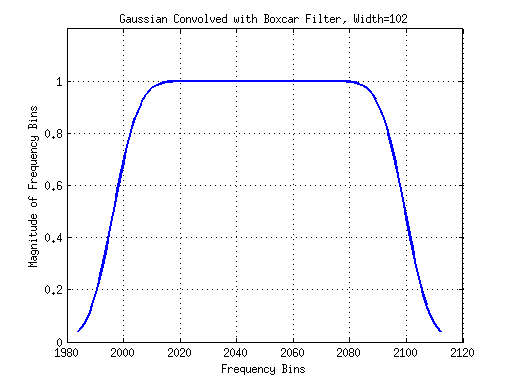
\includegraphics[width=3.3in]{../images/gauss_boxcar.png}
\caption{Box Car \(Width=102\) Convolved with a Gaussian \(\sigma^2 = 50\)}
\label{fig:gauss_boxcar}
\end{figure}

\begin{figure}[h]
\centering
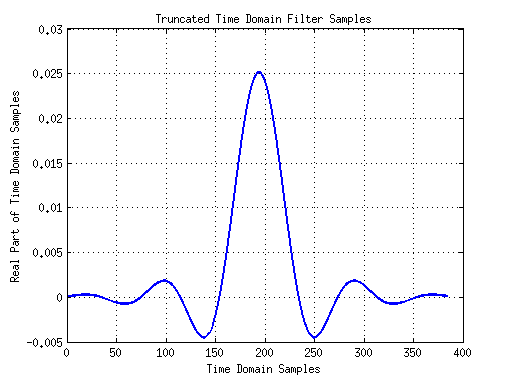
\includegraphics[width=3.3in]{../images/filter_time.png}
\caption{Real Part of Truncated Time Domain Filter \(W=384\)}
\label{fig:filter_time}
\end{figure}

\begin{figure}[h]
\centering
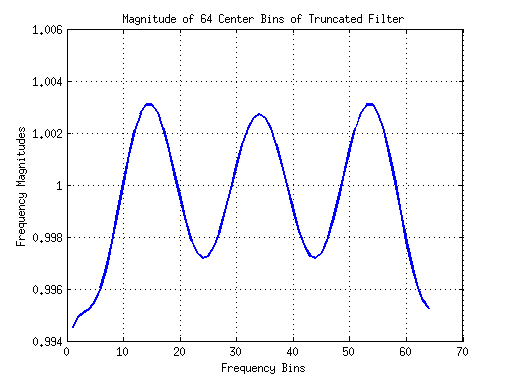
\includegraphics[width=3.3in]{../images/filter_freq.png}
\caption{64 Bins of Truncated Frequency Domain Filter Used for Estimation}
\label{fig:filter_freq}
\end{figure}

\par The inner loop finished by computing the \(B\) point FFT and then finding the top \(dk\) points as shown in figure \ref{fig:z_hat}. These points are linearly mapped back to the frequency range of the input data using the inverse of the permutation found earlier in the loop. The output is the votes for each frequency bin location. An example of the voting space created for a particular run where \(k=6\) is shown in figure \ref{fig:votes}. While the paper uses the top \(L/2\) voted locations, our implementation used the top \(k\) voted locations which seemed to reduce the false alarm rate.

\begin{figure}[h]
\centering
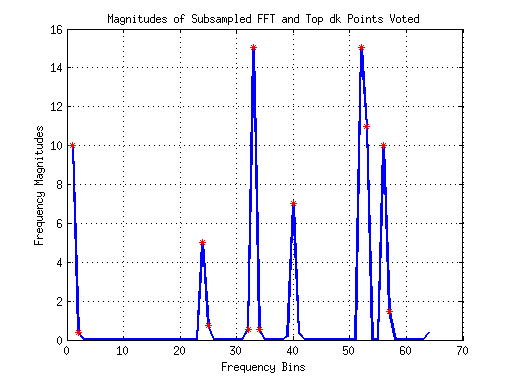
\includegraphics[width=3.3in]{../images/z_hat.png}
\caption{64 Bin Subsampled FFT from One Location Loop Iteration}
\label{fig:z_hat}
\end{figure}

\par The estimation loop proceeds similarly to the location loop and differs in the last step. Instead of votes being cast as in the location loop, the estimation loop computes an estimate to the frequency response at the voted locations as \(\hat{x'}= \hat{z(i)} / \hat{G(i)}\) where \(z(i)\) is the value at the \(i\)th location in the \(B\) point FFT and \(G(i)\) is the corresponding filter value in the frequency domain as shown in figure \ref{fig:filter_freq}.

\begin{figure}[h]
\centering
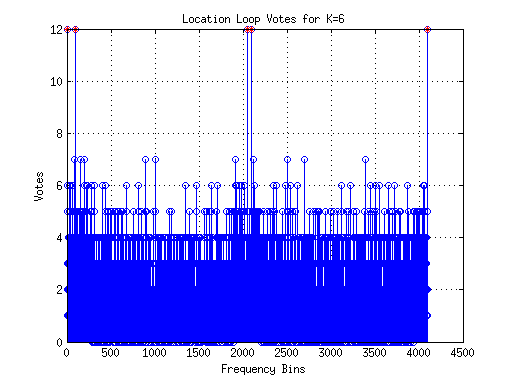
\includegraphics[width=3.3in]{../images/votes.png}
\caption{Votes Made for Each Frequency Bin During Location Loop}
\label{fig:votes}
\end{figure}


\section{Implementation Results}
\par We ran several examples and found the algorithm to be reliably accurate to \(10^{-3}\) precision. We included an example here with a test signal that was created using the frequencies in figure \ref{fig:inputdata}. The phases were all set to zero. These frequencies were put through the Matlab IFFT function and the gain was removed by multiplying by \(n\). Then we ran our implementation and computed the result as plotted in figure \ref{fig:FinalResult}. The frequencies input are in table \ref{table:freqs} and the output frequencies for a different run at in \ref{table:cfreqs}. This example demonstrates the stated precision.

\begin{table}[h!]
\centering
\begin{tabular}{|l|l|l|l|l|l|l|}
\hline
Location  & 1 & 100 & 2048 & 2049 & 2100 & 4096 \\ \hline
Magnitude & 10 & 15 & 5 & 15 & 7 & 10 \\ \hline
\end{tabular}
\caption{Frequency Magnitudes Used in Test Input}
\label{table:freqs}
\end{table}

\begin{table}[h!]
\centering
\begin{tabular}{|l|l|l|l|l|l|l|}
\hline
Location  & 1 & 100 & 2048 & 2049 & 2100 & 4096 \\ \hline
Magnitude & 10.0015 & 14.9925 & 5.0001 & 15.0027 & 6.9953 &  9.9974 \\ \hline
\end{tabular}
\caption{Frequency Magnitudes Computed using SFFT Implementation, All Phases Were Near Zero}
\label{table:cfreqs}
\end{table}

\begin{figure}[h!]
\centering
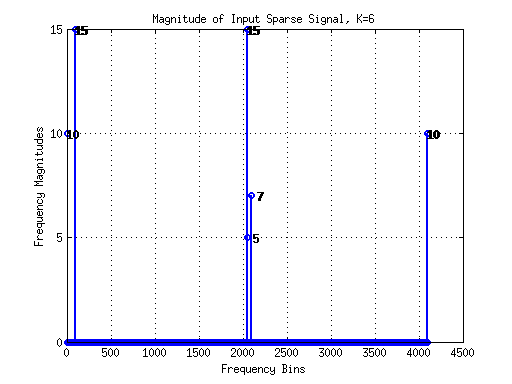
\includegraphics[width=3.3in]{../images/inputdata.png}
\caption{Magnitude of Input Data, Phases All Set to Zero}
\label{fig:inputdata}
\end{figure}

\begin{figure}[h!]
\centering
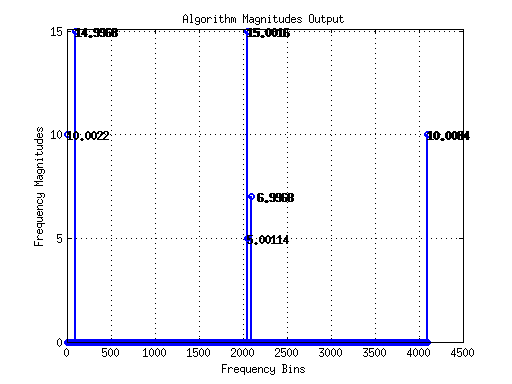
\includegraphics[width=3.3in]{../images/FinalResult.png}
\caption{Estimated Magnitudes from Input Data, Phases All Approximately Zero}
\label{fig:FinalResult}
\end{figure}

\section{Algorithm Performance}
\par To evaluate the algorithm implementation performance, we used the \(L_1\) error just as the original authors of the algorithm did \cite{hass}. The \(L_1\) error computation is in equation \ref{eq:eq1} where \(\hat{x'}\) is the estimated complex frequency and \(\hat{y}\) is the truth. We also computed the false alarm rate to evaluate the algorithm as computed by equation \ref{eq:eq2} where \(FP\) is the number of false positives and \(TN\) is the number of true negatives. These quantities are computed using location only and not the value at those locations because this is accounted for in the \(L_1\) error.

\begin{equation}
Error = \frac{1}{k}\sum_{i=0}^{n}|{\hat{x'_i} - \hat{y_i}}|
\label{eq:eq1}
\end{equation}

\begin{equation}
FAR = \frac{FP}{FP + TN}
\label{eq:eq2}
\end{equation}

\par We evaluated the algorithm performance using the above \(FAR\) and \(L_1\) metrics as a function of increasing sparsity \(k\) and increasing signal-to-noise ratio (SNR). We also ran the algorithm specifically with a sparsity of \(k=1\) to determine at which minimum SNR the algorithm could detect the true frequency. We plotted all the results in figures \ref{fig:kversusl1}, \ref{fig:kversusfar}, \ref{fig:snrversusl1}, \ref{fig:snrversusfar}, and \ref{fig:snrversusl1_k1}.


\begin{figure}[h]
\centering
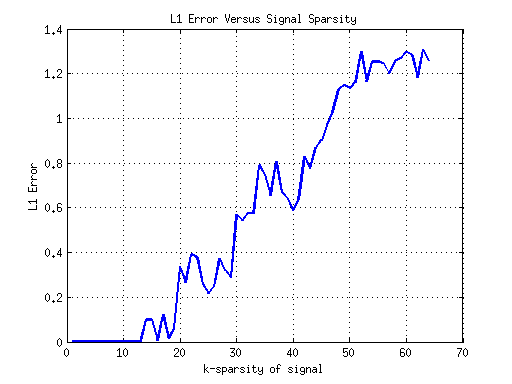
\includegraphics[width=3.3in]{../images/kversusl1.png}
\caption{L1 Error as a Function of Increasing Sparsity \(k=1...64\)}
\label{fig:kversusl1}
\end{figure}

\begin{figure}[h]
\centering
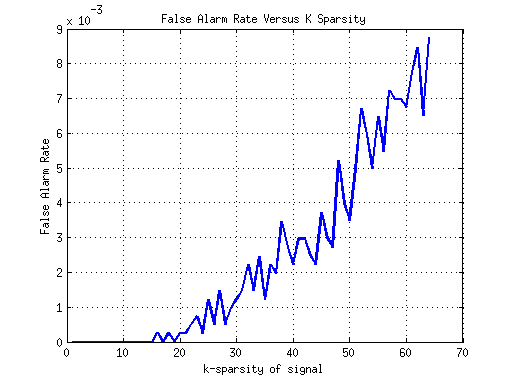
\includegraphics[width=3.3in]{../images/kversusfar.png}
\caption{False Alarm Rate as a Function of Increasing Sparsity \(k=1...64\)}
\label{fig:kversusfar}
\end{figure}

\par In figure \ref{fig:kversusl1} we plotted the \(L_1\) error as a function of increasing signal sparsity \(k\) from \(k=1\) to \(k=64\). Here we see that the error is exceedingly low until \(k\) reaches approximately \(15\). The error increases from there because the permutation step of the algorithm is having difficulties separating the peak frequencies. This is because we are performing a \(B\) point FFT in the location loop and extracting the top \(dk\) samples. These samples are contaminating each other when \(k\) approaches \(B\). We see the same trend in figure \ref{fig:kversusfar}. The \(FAR\) is zero until \(k\) reaches 15. At this point, just as with the \(L_1\) error, the probability of a collision is great enough to cause problems during location finding. The absolute value of the \(FAR\) values is small because of the high number of true negatives \(TN\) in the output. This is expected as the signal is sparse by definition.

\begin{figure}[h]
\centering
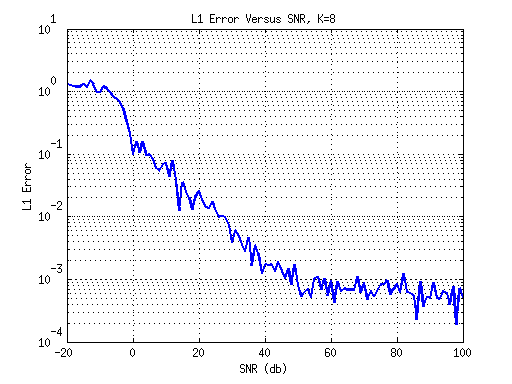
\includegraphics[width=3.3in]{../images/snrversusl1.png}
\caption{L1 Error as a Function of Increasing SNR}
\label{fig:snrversusl1}
\end{figure}

\begin{figure}[h]
\centering
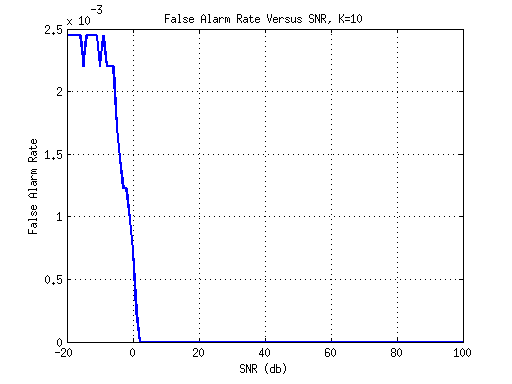
\includegraphics[width=3.3in]{../images/snrversusfar.png}
\caption{False Alarm Rate as a Function of Increasing SNR}
\label{fig:snrversusfar}
\end{figure}

\par In figure \ref{fig:snrversusl1} we plotted the \(L_1\) error as a function of SNR. We used a log scale for the ordinate axis for display purposes only. Here we see that as the SNR increases the \(L_1\) error decreases as expected. This result is in line with the graphic included in the original research paper \cite{hass}. The original paper shows a graphic in which the \(L_1\) error achieved was on the order of \(10^{-7}\) where as our results shows error on the order of \(10^{-3}\). This could be due to implementation issues, but is more likely a function of the input data or filter function. Our data set is considerably smaller than the set used in the paper \(n=2^{22}\) versus \(n=2^{12}\). Also, we used a sparsity of \(k=8\) for this graphic and the original paper uses \(k=55\). In addition, the filter used in the original paper is significantly different from out simple filter. Further testing is needed to see if this is in fact the case.

\par In any case, the graphic does show that when we achieve an SNR about \(-10db\) we see a drop on the \(L_1\) error. We also computed the FAR as a function of increasing SNR and that is plotted in figure \ref{fig:snrversusfar}. We see the same trend as with the \(L_1\) error where the FAR drops considerably at around \(-10db\).

\begin{figure}[h]
\centering
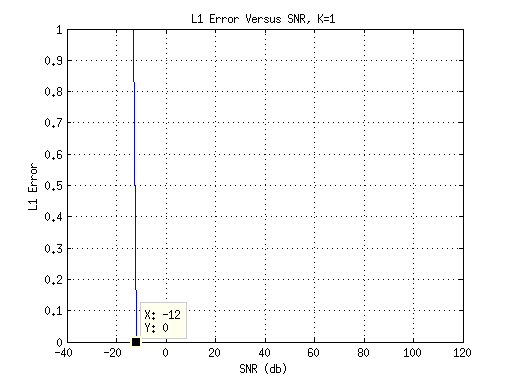
\includegraphics[width=3.3in]{../images/snrversusl1_k1.png}
\caption{L1 Error as a Function of Increasing SNR for \(k=1\) Sparsity}
\label{fig:snrversusl1_k1}
\end{figure}

\par As a final test, we computed the \(L_1\) error as a function of increasing SNR for a signal of sparsity \(k=1\). We wanted to see at what level the algorithm would detect a signal frequency among the noise. We plotted the result in figure \ref{fig:snrversusl1_k1}. From the graph, you can see that our error drops to approximately zero at \(-12db\) and stays near zero for increasing SNR. This is inline with what we found with the preceding tests where the signal sparsity was higher.

\section{Conclusions}
\par After implementing the algorithm, we found that the performance is very good when \(k\) is on the order of about \(1/4B\). Then the algorithm performance falls off approximately linearly until \(k=B\). We also found that the minimum detection threshold is about \(-10db\). Overall, the accuracy is within \(10^{-3}\) when \(n=4096\), \(B=64\), \(k=10\) and \(d=1\). The algorithm is highly dependent on the filter design, choice of \(B\), \(k\) and \(d\) parameters. Therefore, these will need to be tuned for each application domain. The oversampling heuristic parameter \(d\) is critical especially if afrequency magnitude is significantly higher than the others. If a single frequency dominates during the choice of the top \(dk\) peaks in the \(B\) point FFT, see figure \ref{fig:z_hat}, then the smaller frequencies will be ignored. Therefore, when there is a large disparity between frequency magnitudes, then the \(d\) parameter must be increased.

% References section
\nocite{*}
\bibliographystyle{plain}
\bibliography{./references}

% Biography
\begin{IEEEbiographynophoto}{Bernard Lampe}
(M'09) became an IEEE Member (M) in 2009 and received his bachelors of science degree from The University of Michigan in Ann Arbor, Michigan, USA in 2009.
\par Mr. Lampe is also a member of the American Society for Computing Machines (ACM) since 2009.
\end{IEEEbiographynophoto}

% End document
\end{document}

